%----------------------------------------------------------------------------------------
%	SLIDE 3.
%----------------------------------------------------------------------------------------
\begin{frame}
\frametitle{Linux? Unix? GNU? OS???}


\only<1,6>{
\begin{figure}
	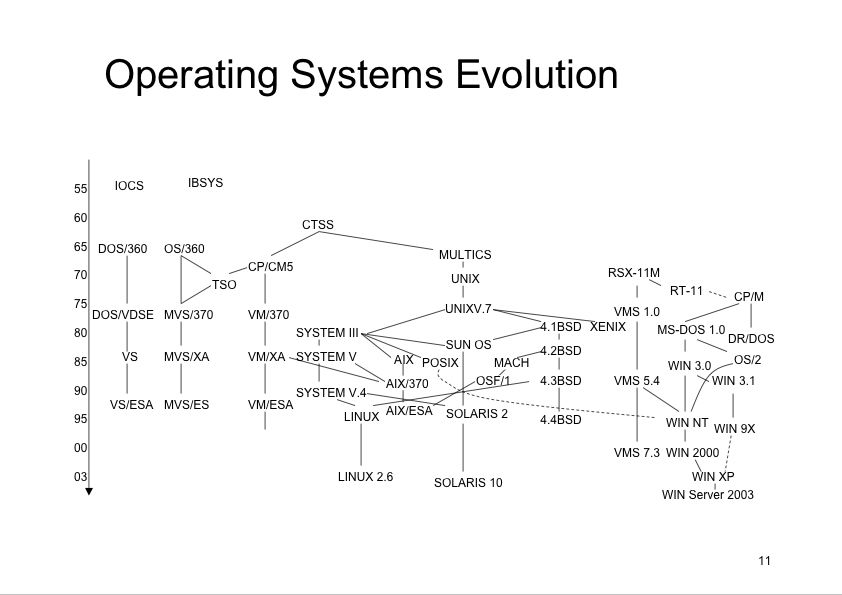
\includegraphics[width=0.85\textwidth]{img/evolution.jpg}
\end{figure}
}


\only<2-4>{
\begin{columns}
	\column{0.45\linewidth}
	\begin{block}{OS}
		\begin{itemize}
			\item<2-> Program that directly manages hardware and provides a unified environment for applications
			\item<3-> First OS were simply I/O systems, but nowadays they are much more intricate
			\item<4-> Three main components:
			\begin{enumerate}
				\item kernel (the heart of the OS)
				\item shell (the interface between the user and the kernel)
				\item basic software and libraries
			\end{enumerate}
		\end{itemize}
	\end{block}

	\column{0.5\linewidth}
	\begin{figure}
		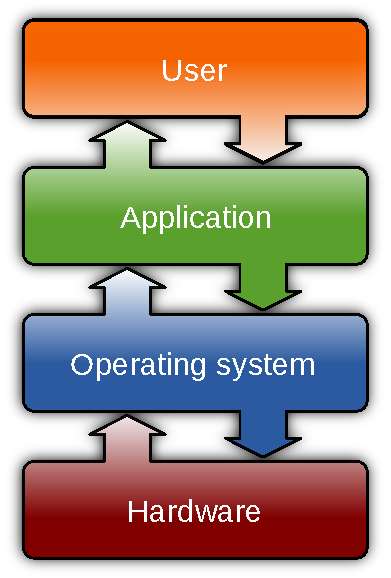
\includegraphics[width=0.8\textwidth]{img/os-en.pdf}
	\end{figure}
\end{columns}
}


\only<5>{
\begin{columns}
	\column{0.45\linewidth}
	\begin{exampleblock}{Booting}
		\begin{itemize}
			\item Nowadays there are more layers between the kernel and the hardware too
			\item UEFI has replaced BIOS-based boot since $\sim 2012$
			\item It's complicated business (POST $\to$ boot loader $\to$ kernel $\to$ OS)
		\end{itemize}
	\end{exampleblock}

	\column{0.5\linewidth}
	\begin{figure}
		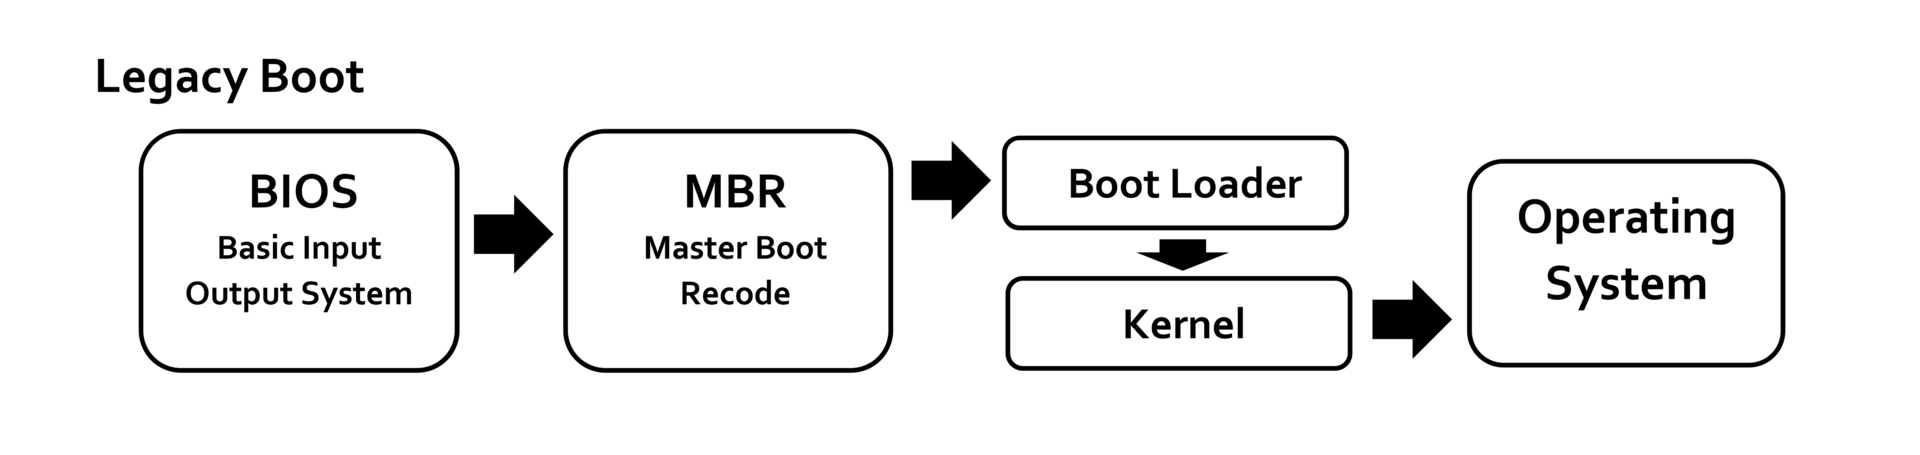
\includegraphics[width=0.9\textwidth]{img/legacy-boot.png}
		\vspace{5pt}
		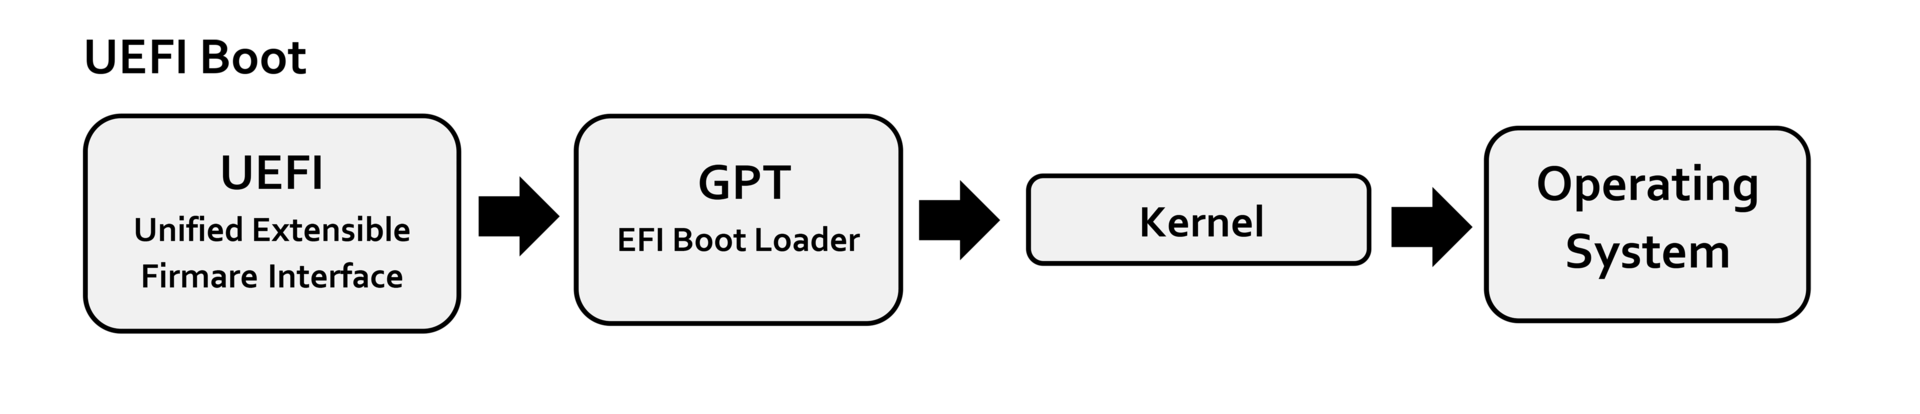
\includegraphics[width=0.9\textwidth]{img/uefi-boot.png}
		\vspace{5pt}
		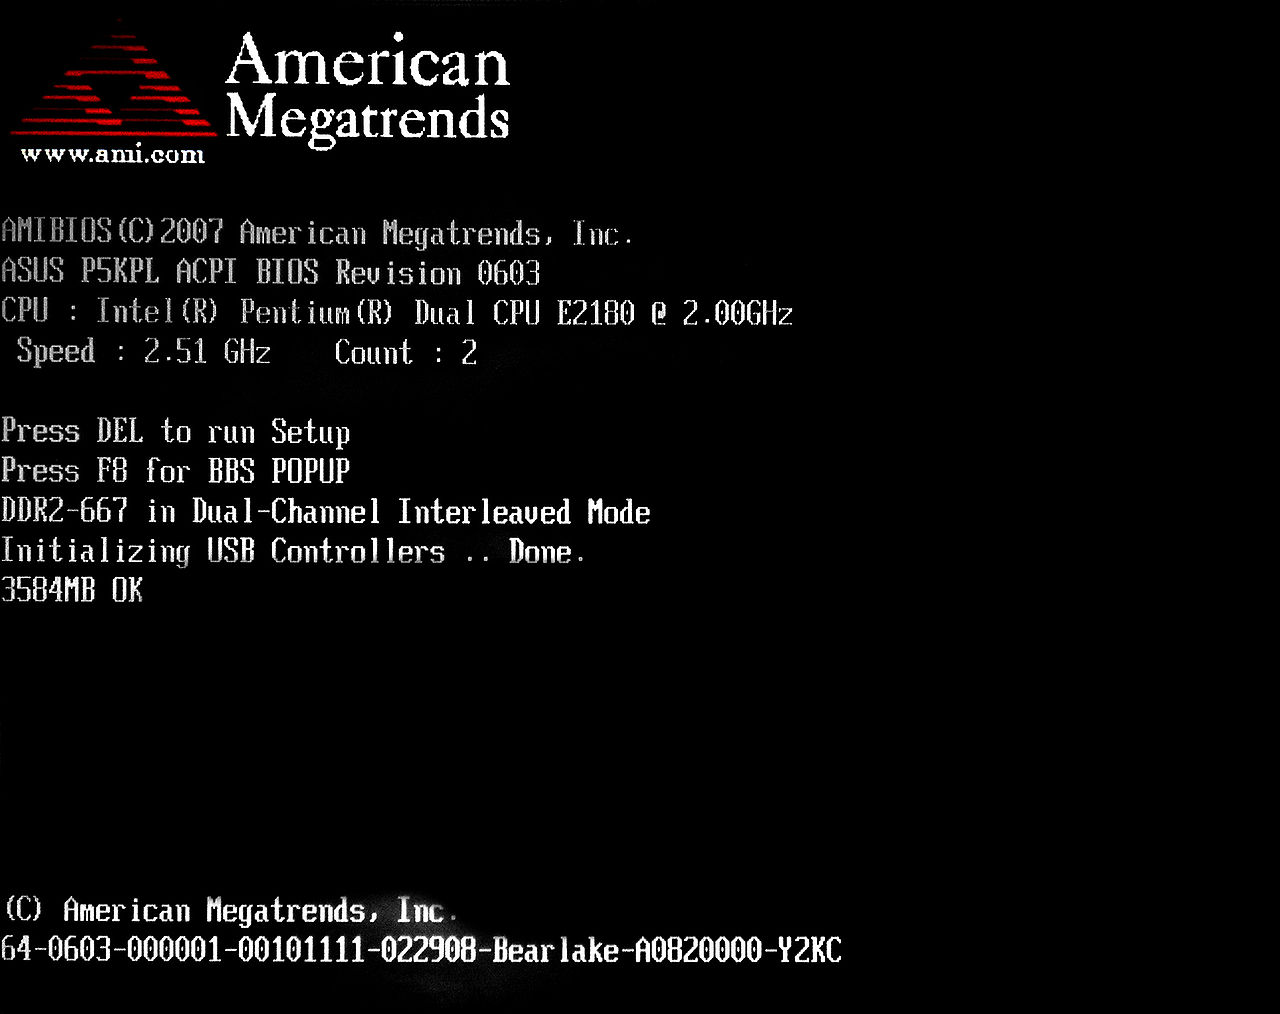
\includegraphics[width=0.9\textwidth]{img/POST.jpg}
	\end{figure}
\end{columns}
}

\end{frame}